\documentclass[a4paper]{article}
\usepackage{tikz, hyperref,comment}
\usetikzlibrary{calc,shapes}
\author{Quang Tung Thai, Namseok Ko, Nopik Park, Meoyngeun Kim}

\title{Toward realizing a cloud-native B5G mobile core architechture}

\begin{document}
\maketitle

\section{Abstract}

The 5G mobile core moved away from monolithic design toward an service based architechture with the network is now being composed of small interacting softwarized components so called network functions. The change is to enable horizental scalability and flexibility in network deployments to meet various vertical use cases with stringent requiements. Going beyond 5G, it is clear that mobile core networks will base on the cloud-native technology with network functions being deployed in multiple distributed clouds. This paper discusses limitations of the current core architechture with a forward looking to its cloud-native realization. In order to completely adopt the cloud-native culture, the architechture should be restructured to enable a clear separation between the development and deployment of mobile network applications.  Following this vein, we make a holistic architechtural change to the core by moving some of it parts into a integartion fabric layer. We discuss how the fabric is design and its benefits to the development of the beyond 5G core network.



\section{Introduction}

The 5G mobile network was designed to support various types of applications with different stringent requirements.  With the small cell ... and machine-to-machine communication, the signaling traffic at the network core is very crowded. 

Further more, many vertical applications would need the concept of multi-domain slicing where a slice can span several domains of different administratives. How to isolate the network function in different slices and how the network function in a slice can communicate accross domains are fundamental question that need ...

In order to meet those requirement, the 5G adopts the Service Based Architechture (SBA) that decomoposes the network into small software network functions. 
Network functions should be implemented without concerning of how they are deployed, that is, the logic for service discovery and selection should be separated from the functional logic.

\begin{comment}

Shifting to Network Disaggregation with a Service-Based Architecture

Service providers are defining and deploying a cloud-native infrastructure across the entire network from the core to the far edge. As defined by the 3rd Generation Partnership Project (3GPP), a Service-Based Architecture (SBA) is a set of interconnected network functions (NFs) that deliver the control plane functionality and common data repositories of a 5G network. Supporting a cloud-native SBA brings new requirements for the control, coordination, and orchestration of disaggregated network functions that are distributed across the network. Network functions are containerized microservices that can support the 5G Core, virtualized radio access network (vRAN), and the N6-LAN network functions.


Cloud-native, service-based architecture introduces a paradigm shift that enables service providers to migrate from a vertical to a horizontal stack implementation. A vertical stack approach increases vendor lock-in and requires that each vendor enables its own infrastructure, increasing complexity.

A horizontal stack approach breaks such vendor complications and limitations while enabling the service provider to maintain control and visibility of its network. With a horizontal stack, service providers gain a consistent cloud-native infrastructure (telco cloud) implemented across core, edge, and far-edge sites—supporting vRAN, a standalone (SA) 5G Core, internal applications, and enterprise- and consumer-facing applications 5G allows service providers to move to a horizontal stack approach, making it possible to scale edge sites as needed for subscribers.



F5 Carrier-Grade Aspen Mesh helps service providers improve application traffic visibility, security, and policy management. The service mesh is designed specifically for service provider cloud-native infrastructures and is built on the open source platform Istio with added features critical for a service provider network. F5 Carrier-Grade Aspen Mesh delivers:

Traffic visibility at all layers through a view of traffic within each 5G Core Kubernetes cluster. This provides revenue assurance and visibility into the data needed to monetize 5G using existing billing systems.
Advanced security with a consistent approach for encrypting and authenticating all traffic between multi-vendor and multi-site networks functions. F5 Carrier-Grade Aspen Mesh is built on techniques based on a carrier-grade and 3GPP-compatible certificate authority.
Traffic control and policy management that enable service providers to efficiently route service communication—and enforce business and compliance policies for the service mesh and network traffic. 
In addition to these features, F5 Carrier-Grade Aspen Mesh provides packet capture capabilities, which standard Kubernetes does not. Packet capture is important for troubleshooting communication issues between CNFs within the cluster and to support governmental requirements such as lawful intercept.

5G networks are poised to deliver high bandwidth, low latency, and faster performance—both driving and enabling application innovation and new business models. To deliver cost-effective 5G performance, service providers are taking advantage of the microservices-based, cloud-native containerized architecture already in use by enterprises. These new solutions give service providers the ability to dynamically place workloads within a network and build out their MEC platform to support the next generation of applications.

Leading-edge solutions from F5 help service providers deliver new 5G functionality while maintaining their existing 4G core networks. F5 BIG-IP Next Service Proxy for Kubernetes (SPK) and F5 Carrier-Grade Aspen Mesh enable service providers to maintain real-time application visibility, scale to meet demand, and increase traffic visibility and security. F5 N6 LAN solutions help service providers deliver network functions, reducing cost and improving performance. These solutions work in conjunction with F5 security solutions designed to protect networks from new attack vectors and threats. With the right solutions in place, service providers can take advantage of the many benefits of a cloud-native infrastructure from the core to the far edge of the network as they embark on the 5G journey. 



\end{comment}


Are we realy cloud-native yet?
The cloud-native with CI/CD and Depob culture allows IT industry moving forward in fast pace. (Make it clear about CI/CD).

In contrast, the telco world has been moving slowly. .....



The fundamental principal in microrchitechture is a clear separation between development and operation. The developers of a project should only focus on the bussiness logic to enable the application functions. They working process should not ... with the scalability, security .

The current 5G architechture have a complete ...., how ever the boundary between the two process is blurr. 

The need to break away from connection (endpoint)-based protocol design mindset. For example, in service registration and discovery, multiple NRF can be deployed and NRF can forward a discovery query to another NRF. However, the standard does not specify on which condition the NRF should ask the other NRF....

On the otherhand, the cloud-native movement has been progress quickly over the years. 
... However, how to fit the current core network architechture into the current Kubernetes infrastructure is not trivial. In this work, we argue that there a ovelapping areas between the 5G sppecifications and the current architechture of Kubernetes ecosystems. There redundancy must be resolved in order for the telco to fully take advantage of the technological progress which has beend accumulated in the cloud-native community.

In line with that argument, we propose several modification to the current 5G network architechture. We stress that within the signaling network of the mobile core, there must be a clear separation between control plane and data plane. The data plane is what the traffic move between functional network function to support the telco applications. On the otherhand, the control plane represent the control signal that operate the network to adapt to dynamic demands. This separation is 



\section{Analysis of current architechture}

\subsection{Service discovery and selection}

Service registration and discovery is a common pattern in microservice architechture. There are an abundancy of approaches ... The 5G specifications have a simple ... We believe that this operational ..

Another pitfall of current approach in 5G specifications is that it is open for cross domains service discovery. That is, a service in one domain can request the NRF from another domain to look for suitables services. This method exposes two problems: first, it requires a security mechanism to protect the requested domain from unexpected requests; second, the logic for sevice discovery can become complex as there is no boundary on the number of NRF to be queried.


Setting a stadard for the implementation of a non-function feature may be hurtful to the development of innovative ideas. 
The service discovery is vital for the system operation. Is is therefore should be implemented with stringent requirements. Availability, resiliency and security should be guaranteed. There could be various methods to fulfil the requirements as it can be seen in the current microservice community.


NRF is not a mandatory network function as the core network can be configured manually. For example, and AMF may have a list of network addresses to the available SMFs in its configuration for selection. However, if the operators want to provision the network functions regarding to demands or execute/turn off network functions on-demand, this method is not suitable. Therefore, unless the network is configured for testing, the NRF is a crictical component of the network.

In current standard, a network function need to discovery the location of a service it wants to requests through the NRF. The network function should be configured with a fixed location of the NRF. All network functions should register its profile with the NRF and periodically send a heartbeat signal to update its status. 



This approach has several drawbacks. First, the selection is dependent on the network operator policy. The specification (ref) does not specify how precisely an NF select another NFs. It recommends a set of parameters which can be used in the query so that the NRF can create a filter to search for appropriate NFs. This is a troublesome as different vendor may implement the feature differently. We may hope that the policy is not hardcoded into the source-code, instead it should be configurable. Even so, the diversity of configuration methods is also a big issue for the operators.
Second, the NRF can be a single point of failure and it can be a source of signaling traffic congestion.



\subsection{Service communication proxy}

Since release 16, 3GPPP introduced the SCP (service communication proxy) network function. It is an optional component, that means the core network should be functioning without the SCP. 
There are several problem with the introduction of the SCP. First, it is not clear when the SCP should be used. The network functions can choose several communication modes: whether request/response should be go through SCP; or whether network function selection should be delegrate to the SCP. 
\textcolor{orange}{to be updated}

\section{Towards a cloud-native deployment of the core network}
\subsection{Kubernetes and service mesh}

In this section, we briefly introduce the Kubernetes, a container orchastration platform and the concept of service mesh for microservice architechture.

Kubernetes is an opensource orchastration system that enables automation deployment of contenerized applications on a cluster of machines. It was designed to manage the life cycle of applications and services in a method that provides predictability, scalability, and high availability.

When an operator needs to deploy an application consiting of microservices on a K8 cluster, he may state a desireable state of his deployed system through a specification. The K8 schedule always monitor the status of the deployment and try to make sure that it is matched to the desired state.

The basic element of a Kubernetes system is a pod which can be regarded as a virtual host with isolated resouse running on a cluster computing node. Applications can be contenerized and initiated on a pod. They are sharing the same life cycle as the pod itself.


As microservices in Kubernetes are scheduled dynamically, thei locations are ephermaral. A service must find the location of other services that it wants to request. Kubernetes support service registration and discovery natively. In short, when a ...

\textcolor{orange}{to be updated}
\subsubsection{Service mesh for 5G}

Why the current service mesh solotion is maturing and become more and more useful in cloud platforms, they are not suitable to the current 5G architechture. It is due to two reasons: first, the current 5G core architechture already include the service registration and discovery part, therefore, it does not need a service mesh. But event if one might ignore the NRF deployment to opt for the service mesh approach, it raises another issue: the sidecar proxy introduce another extra hop in the signaling path. Also the signaling packet must be handled at the proxy. In all, they migh introduce a significant latency to the delivery of signalling packets. This can be ...


\textcolor{orange}{to be updated}
\subsection{B5G aware cloud-native service mesh}

In previous sections, we argue that current 5G architechture is still a work in-progress toward a cloud-native platform. There is a overlaping between application logic and operation which makes it still difficult to developed and deployed. On the other hand, the current service mesh solutions are not suitable for the requirements of the next generation mobile network architechtures. Therefore, in this work we propose a new service mesh architechture that is B5G aware. 



\subsubsection{Overall architechture}

We adopt the cloud-native philosophy to re-architech the mobile core network to enforce a clear separation between the implementation of network functions and network operation. Some network functions and core procedures will move to a integration fabric. The fabric is responsible for deployment of services and routing requests among the services. The bussiness logic within network functions therefore can be simplified since the fabric helps routing requests to appropriated destination and collecting their responses. 

A service mesh fabric operates on a single cluster. It consists of a centralized service controller and service agents which are illustrated on the Figure \ref{fig1}. The NRF, NSSF and SCP components in the original 5G architechture is completely removed. Their responsibility, that is to support a comsumer to select an appropriate instance of a target service within an application context, is relialized by the service controller working in tandem with the service agents. In addition, common logic for NF discovery and selection implemented at consumers are moved into the service agent. The agent is acting as a proxy that do the request and response on behalf of the network functions. It abstract away all the service registration/discovery an subscribe/notification procedures from the network functions. The service agents communication with the service controller for service registration and discovery and install routing rules onto the agents. 

A network function is built upon a common service routing library (service agent). The library provides simple unified interface for sending and receving request which is used by all the network functions. 

In order to support deployments that span accross multiple domains, such as the cases of multi-domain slicing, gateway compoments are introduced. A gateway is a special network function that connects its domain to others. Similar to the others network function, it is built upon the service agent and recieved routing rules from the service controller to forward requests and respones accross domains. When an agent has an request that targets a cross-domain service, the request is forward to a gateway outbounding to the target domain cluster.

%\begin{center}
%\includegraphics[width=\textwidth]{agent-controller}
%\end{center}

\begin{figure}[h!]
  \begin{center}
	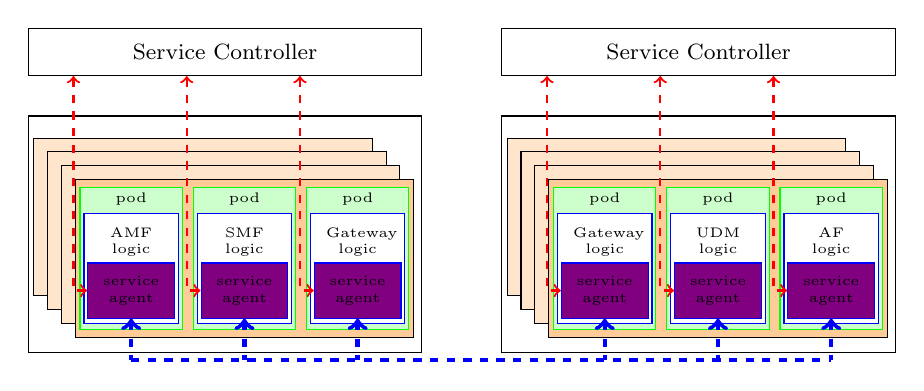
\begin{tikzpicture}[bound/.style={rectangle, draw=black,inner sep=0, fill=white, minimum width=5cm, minimum height=0.6cm,font=\footnotesize},
	cnode/.style={rectangle,draw=black,fill=orange!20, minimum width=4.3cm, minimum height=2cm},
	pod/.style={rectangle, inner sep=0, fill=green!20,draw=green, minimum width=1.3cm, minimum height=1.8cm},
	nf/.style={rectangle, inner sep=0, fill=white,draw=blue,minimum width=1.2cm, minimum height=1.4cm,above,yshift=2pt},
	agent/.style={rectangle, inner sep=0, fill=violet,draw=blue,text width=1.1cm, minimum height=0.7cm, font=\tiny, align=center},
	nflab/.style={text width=0.8cm,font=\tiny,align=center, inner sep=0},
	clink/.style={thick, red, dashed},
	dlink/.style={ultra thick, blue, dashed}]

		%controller
		\node[bound] at (0,0) (c1) {Service Controller};
		\node[bound,right] at ([xshift=1cm]c1.east) (c2) {Service Controller};
		%network functions
		\node[bound,minimum height=3cm,below] at ([yshift=-0.5cm]c1.south) (d1) {};
		\node[bound,minimum height=3cm,below] at ([yshift=-0.5cm]c2.south) (d2) {};
		
		\node[cnode,below] at ([yshift=-8pt,xshift=-8pt]d1.north) (n11) {};
		\node[cnode] at ([yshift=-5pt, xshift=5pt]n11) (n12) {};
		\node[cnode] at ([yshift=-5pt, xshift=5pt]n12) (n13) {};
		\node[cnode,fill=orange!40] at ([yshift=-5pt, xshift=5pt]n13) (n1) {};
		
		\node[cnode,below] at ([yshift=-8pt,xshift=-8pt]d2.north) (n21) {};
		\node[cnode] at ([yshift=-5pt, xshift=5pt]n21) (n22) {};
		\node[cnode] at ([yshift=-5pt, xshift=5pt]n22) (n23) {};
		\node[cnode,fill=orange!40] at ([yshift=-5pt, xshift=5pt]n23) (n2) {};
		\foreach \i in {1,2} {
			\node[pod] at ($(n\i.west)!0.1666!(n\i.east)$) (pod\i1) {};
			\node[pod] at ($(n\i.west)!0.5!(n\i.east)$) (pod\i2) {};
			\node[pod] at ($(n\i.west)!0.8333!(n\i.east)$) (pod\i3) {};
			\foreach \j in {1,2,3} {
				\node[below,yshift=-2pt,font=\tiny, inner sep=0] at (pod\i\j.north) {pod};
			}
		}
		
		\foreach \i in {1,2,3} {
			\node[nf] at (pod1\i.south) (nf1\i) {};
			\node[agent,above] at ([yshift=2pt]nf1\i.south) (agent1\i) {service agent};
			\node[nf] at (pod2\i.south) (nf2\i) {};
			\node[agent,above] at ([yshift=2pt]nf2\i.south) (agent2\i) {service agent};
		}
		\node[nflab,above] at ([yshift=2pt]agent11.north) {AMF logic};
		\node[nflab,above] at ([yshift=2pt]agent12.north) {SMF logic};
		\node[nflab,above] at ([yshift=2pt]agent13.north) { Gateway logic};
		\node[nflab,above] at ([yshift=2pt]agent21.north) {Gateway logic};
		\node[nflab,above] at ([yshift=2pt]agent22.north) {UDM logic};
		\node[nflab,above] at ([yshift=2pt]agent23.north) { AF logic};
		\foreach \i in {1,2} {
			\foreach \j in {1,2,3} {
				\draw[dlink,<-] (agent\i\j.south) -- ++ (0,-15pt);
				\draw[clink,<->] (agent\i\j.west) -- ++(-5pt,0) coordinate (ttp\i\j) -- (ttp\i\j |- c\i.south);
			}
		}
		\draw[dlink] ([yshift=-15pt]agent11.south) -- ([yshift=-15pt]agent23.south);
	\end{tikzpicture}
  
  \caption{B5G native service mesh  \label{fig1}}
  \end{center}
\end{figure}




\subsubsection{Service mesh composition}

In this section, we further detail the composition of the service mesh by disecting it into smaller components to describe their roles and interactions. The composition is shown on Figure \ref{fig2}. At the top of the figure is the service controller which consists of four components in yellow color. The lower blue boxes represent network functions.

A network function composes of its busseness logic part and a service agent. The service agent provide APIs for requesting service and responding to requests. The agent executes service discovery and selection and hide these procedures from the bussiness layer. The agent therefore belongs two both control plane and data plane. On the data plane, it routes request/respone toward other agents. On the control plane, it interacts with the service controller to dynamically update internal routing rules.

The \textit{Forwarder} is the core module of the service agent on the data plane part. On one hand, it intefaces with the bussiness logic part to handle its requests and responses. On the other hand, it maintains a list of transport connections to the other service agents to forward outgoing and receiving incomming requests and responses. The \textit{configuration} component keep information that defines how the service agent should behave. it may have a list of static connection information to other service agents, a defaul policy to select a network function from a list of candidates.

The \textit{Service Discovery} component relializes all procedures for notifying of the network function to the fabric and discovery other network functions of interests. It interacts with the \textit{Service broker} component of the sercice controller to keep synchronizing with the whole mesh. When the \textit{Forwarder} needs to forward a request to a new remote service, it asks the \textit{Service Discovery} component for a list of candidate locations of the target service then selects one of the candidate to make a connection for sending the request. The \textit{Selection} component implements load balancer algorithms to make the selection. It is the the \textit{Policy Manager} component at the service controller that chooses the load balancing algorithm to be used at the service agent.

The \textit{Secured connection} component at the service agent working in tandem with the \textit{security manager} at the service controller to create secured connections betweern service agents. The \textit{Security manager} might generate a private key and sign a corresponding certificate for the agents and distributes the certificate to the agents. The agents then use the information to establish secured connections for delivering the data plane traffic.

Finally, the \textit{telemetry} component at the agent and the \textit{Telemetry manager} component at the controller provides the observability for the service mesh. Since all the signalling traffic among network functions is channeled through the service agents, the \textit{telemetry} component might collect statistics of the traffic then make them available for serving to the network. The \textit{Telemetry manager} specifies what telemetrical data to be collected at the agents and it may also pull the data from them for data analytics.

%\begin{center}
%\includegraphics[width=0.6\textwidth]{agent-nf}
%\end{center}

\begin{figure}
\begin{center}
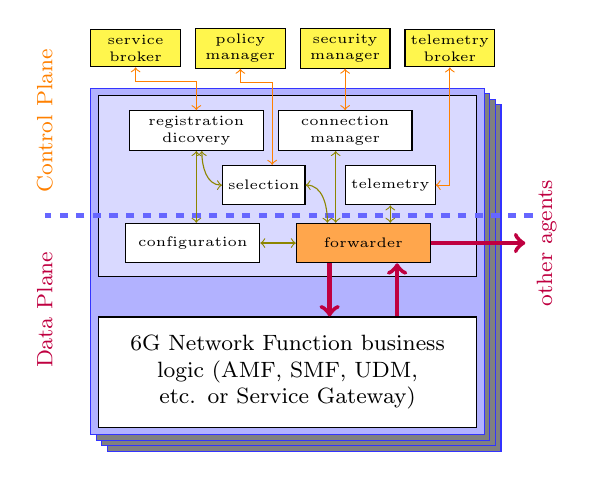
\begin{tikzpicture}[comlab/.style={font=\tiny\linespread{0.6},align=center,inner sep=2pt},
ccom/.style={rectangle,draw=black,fill=yellow!70,text width=1cm},
dcom/.style={rectangle,draw=black,fill=white, minimum height=0.5cm},
nf/.style={rectangle,draw=blue!80,fill=black!50,minimum width=5cm,minimum height=4.4cm}]
	%network functions
	\node[nf] at (0,0) (nf4) {};
	\node[nf] at ($(nf4)+(-2pt,2pt)$) (nf3) {};
	\node[nf] at ($(nf3)+(-2pt,2pt)$) (nf2) {};
	\node[nf,fill=blue!30] at ($(nf2)+(-2pt,2pt)$) (nf1) {};
	%controller
	\node[comlab,ccom,right] at ([yshift=0.5cm]nf1.north west) (c1) {service broker};
	\node[comlab,ccom,right] at ([xshift=5pt]c1.east) (c2) {policy manager};
	\node[comlab,ccom,right] at ([xshift=5pt]c2.east) (c3) {security manager};
	\node[comlab,ccom,right] at ([xshift=5pt]c3.east) (c4) {telemetry broker};
	%nf logic
	\node[minimum width=4.8cm, minimum height=1.4cm, fill=white, draw=black] at ([yshift=0.8cm]nf1.south) (nfb){};
	
	\node[text width=4.5cm, inner sep=4pt, align=center,font=\footnotesize] at (nfb) {6G Network Function business logic (AMF, SMF, UDM, etc. or Service Gateway)};
	
	%agent
	\node[minimum width=4.8cm, minimum height=2.3cm, fill=blue!15, draw=black,above] at ([yshift=0.5cm]nfb.north) (ag){};
	
	\node[dcom, comlab, above, minimum width=1.7cm] at ([yshift=5pt]$(ag.south west)!0.25!(ag.south east)$) (conf) {configuration};
	\node[dcom, comlab, fill=orange!70, above,minimum width=1.7cm] at ([yshift=5pt]$(ag.south west)!0.7!(ag.south east)$) (fwd) {forwarder};
	\node[dcom, comlab, below,minimum width=1.7cm, text width=1.5cm] at ([yshift=-15pt]c3.south) (sec) {connection manager};
	\node[dcom, comlab, left, minimum width=1.7cm, text width=1.5cm] at ([xshift=-5pt]sec.west) (disc) {registration dicovery};

	\node[dcom, comlab, below] at ([yshift=-5pt]disc.south east) (sel) {selection};
	\node[dcom, comlab, right] at ([xshift=0.5cm]sel.east) (tel) {telemetry};
	
	\draw[<->,orange] (c1.south) -- ++(0,-5pt) -| (disc.north);
	\draw[<->,orange] (c2.south) -- ++(0,-5pt) -| ($(sel.north west)!0.6!(sel.north east)$);
	\draw[<->,orange] (c3.south) -- (sec.north);
	\draw[<->,orange] (c4.south)  |- (tel.east);
	\coordinate (p1) at ($(fwd.south west)!0.25!(fwd.south east)$);
	\coordinate (p2) at ($(fwd.south west)!0.75!(fwd.south east)$);
	\draw[->,ultra thick, purple] (p1) -- (p1 |- nfb.north);
	\draw[<-,ultra thick, purple] (p2) -- (p2 |- nfb.north);
	\draw[->,ultra thick, purple] (fwd.east) -- +(1.2cm,0) node[below, rotate=90, align=center] (p3) {\footnotesize other agents};
	\draw[ultra thick, blue!60, dashed] ($(p3)+(-5pt, 10pt)$) -- ++(-6.2cm,0) coordinate (p4);
	\node[rotate=90,orange] at ([yshift=1.2cm]p4) {\footnotesize Control Plane};
	\node[rotate=90,purple] at ([yshift=-1.2cm]p4) {\footnotesize Data Plane};
	\draw[olive,<->] ([xshift=2pt]disc.south) to[out=-90,in=180] (sel.west);
	\draw[olive,<->] (disc.south) -- (disc.south |- conf.north);
	\draw[olive,<->] (conf.east) -- (fwd.west);
	\draw[olive,<->] (tel.south) -- (tel.south |- fwd.north);
	\coordinate (fwd1) at ([xshift=-10pt]fwd.north);
	\coordinate (fwd2) at ([xshift=-3pt]fwd1);
	\draw[olive,<->] (fwd1) -- (fwd1 |- sec.south);
	\draw[olive,<->] (fwd2) to[out=90,in=0] (sel.east);
\end{tikzpicture}

\end{center}
\caption{Functional components of the proposed B5G-aware service mesh}
\label{fig2}
\end{figure}

\subsection{Network function identification}

In cloud-native approach, each service is a long-lived name that exists uniquely within the namespace of its application. It is the service mesh that maintains a mapping of the name to the location of a service instance. Business logic of the  application therefore is constructed using these service names instead of the location of its deployed instances.
In the 5G mobile core network, a network function may provide multiple services (with different service names). In order to separate the business logic from the application deployment there must be a mechanism to maintain a static identification of the network function. This is to enable the services to be requested without awareness of the network function deplotment.

The current 5G standard does not explicitly specify how a network function is identified. Unfortunately, it is hardly possible to assign a static name to a network function. The reason is that a network function may exist in multiple application scopes. For example, an AMF may belong to different network slices, therefore, living in different contexts. 


- using query to identify a network function
- the closeness of NRF
- How to open the concept so that the integration fabric can accept new applications (new network function) -> generalized the concept of identification

For realizing this scheme, we introduce the concept of application context. It is defined as a logocal setting where a group of network functions interact to make sense of certain application logic. Examples of the context may includes a PLMN, a DNN, a network slice, a network slice instance. etc. 

 

Contexts may be ovelapping; that means a single network function may be included in multiple contexts. For example, an AMF may be a share network function among multiple network slices. We assume that each context can be specified with a context description using a well-defined format. In an operating network environment, a network function type and a context therefore uniquely identify a set of network function instances of the same type. These instances are identical in terms of supporting the applications in the same context.

A context should be defined by network operators and it is 


\subsubsection{Agent - Network function logic interface}

Having introduce the concept of application context, it is now simple to define the interface exposed by the service agent to the business layer of a network application.



\subsubsection{Distributed service registry}

The separation of sevice selection and discovery from bussiness logic of the network functions brings a great benefit in terms of realizing the network architechture. It enables various approaches for implementing the service routing. In this work, we propose a distributed service discovery platform that is more responsive and more scalable than current approach which is based on NRF interface.

Here, the service agents can manage partial registry data which is relevant to the network function they are serving. The service controller is not a centralized registry, instead, it works as a registry broker which notifies the service agents of relevant new registrations. This approach removes the bottleneck issue which may occur in the current architechture with NRF as the centralized service registry. In addition, a network function can discovery the location of a service in instance because the service agent is co-located and it has all neccessary registry data.

Figure \ref{fig3} illustrated a common procedure of service registration and registry update at agents. In the example, there are three agents: the agent 1 is a newly initiated and it needs to announce its existance to the service mesh while the other two remaning agents already announced. Suppose that the deplopyment have three context C1, C2. The agent 1 and 3 are operating in context C1 while the agent 2 is operating in context C2.

When the network function instance attached to the service agent 1 is initiated, the agent itself announces to the service controller (1). The transport address of the controller should be known by the service agent as the information is set up by the operators when configuring the network function.  The announcement should include following pieces of data: a) the transport address of the agent; b) a list of context where the network function operates (L10); c) and a list of context of interest (L1i). The context lists are application logic's dependent.The list in c) is to tell the service controller the intention to listen to the membership changes in listed contexts. 

The service controller maintain the list of all network function instances which have been announced; and it also keeps track of their contexts as well as the contexts they wish to monitor.

Upon receiving the request, the controller response with a list of locations of network function instances which belong the the interested contexts which was expressed by the requester. For example, the agent 1 includes context C2 in its interested list, the controller should include the address of the agent 3 in the response.

At the same time, the controller notifies all network function in the context C2 (and other contexts in L1i). The agent 3 should be received the notification (supposed that it is also interested in the C2 context updates).

The agent 1 extract the list of announced agents in the response from the controller then send a request to each of them for retriving their profiles (4). Similarly, the agent 3 also send a request to agent 1 to pull its profile (6). Upon receiving a request, a receiving agent should response with its profile (5 and 7).


\begin{figure}[h!]
\begin{center}
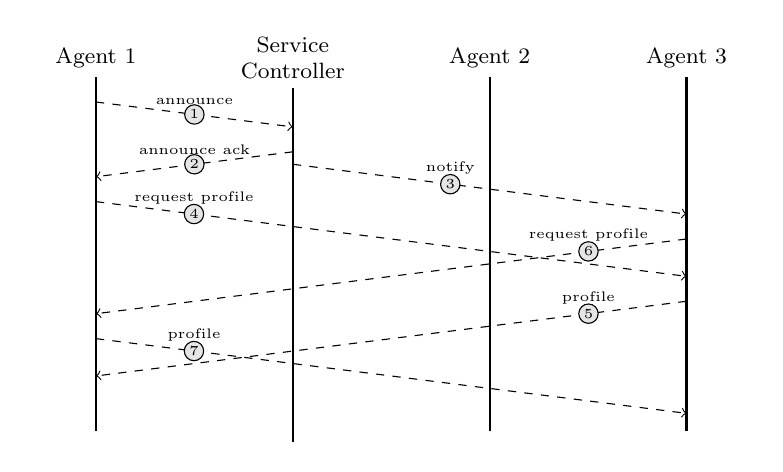
\begin{tikzpicture}[lab/.style={font=\footnotesize\linespread{0.8},text width=1.5cm,align=center},
axis/.style={thick},
link/.style={->, dashed},
linklab/.style={draw,circle,minimum width=7pt,fill=black!10,inner sep=0,font=\tiny},
msg/.style={above,font=\tiny}]
	\def\xx{2.5cm}
	\def\yy{-9pt}
	\def\ll{-4.5cm}
	\node[lab] at (0,0) (f1) {Agent 1};
	\node[lab] at ([xshift=\xx]f1) (f2) {Service Controller};
	\node[lab] at ([xshift=\xx]f2) (f3) {Agent 2};
	\node[lab] at ([xshift=\xx]f3) (f4) {Agent 3};	

	\draw[axis] (f1.south) -- +(0,\ll);
	\draw[axis] (f2.south) -- +(0,\ll);
	\draw[axis] (f3.south) -- +(0,\ll);
	\draw[axis] (f4.south) -- +(0,\ll);

	%register
	\draw[link] ([yshift=\yy]f1.south) -- node (l1) {} ++(\xx,\yy) coordinate (p1);
	%response
	\draw[link] ([yshift=\yy]p1) -- node (l2) {} ++(-\xx,\yy) coordinate (p2);
	%notify
	\draw[link] ([yshift=1.5*\yy]p1) -- node[pos=0.4] (l3) {} ++(2*\xx,2*\yy) coordinate (p3);
	%pull
	\draw[link] ([yshift=\yy]p2) -- node[pos=0.166] (l4) {} ++(3*\xx,3*\yy) coordinate (p4);
	%pull-response
	\draw[link] ([yshift=\yy]p4) -- node[pos=0.166] (l5) {} ++(-3*\xx,3*\yy) coordinate (p5);
	
	\draw[link] ([yshift=\yy]p3) -- node[pos=0.166] (l6) {} ++(-3*\xx,3*\yy) coordinate (p6);
	%pull-response
	\draw[link] ([yshift=\yy]p6) -- node[pos=0.166] (l7) {} ++(3*\xx,3*\yy) coordinate (p7);
	
	\foreach \i in {1,...,7} {
		\node[linklab] at (l\i) {\i};
	}
	\node[msg] at (l1) {announce};
	\node[msg] at (l2) {announce ack};
	\node[msg] at (l3) {notify};
	\node[msg] at (l4) {request profile};
	\node[msg] at (l5) {profile};
	\node[msg] at (l6) {request profile};
	\node[msg] at (l7) {profile};
\end{tikzpicture}
\caption{Service registration}
\label{fig3}
\end{center}
\end{figure}




\section{Conclusion}

In this work, we anlyzed the current 5G core network architechture and identified its limitations in terms of realizing a cloud-native deployment. We proposed the separation of control plane and data plane in the signaling network. (harmonizing with the service mesh archichture in cloudnative platform). Specifically, network functions interacts in the data plane to fulfil the mobile application bussiness. However, how the signaling traffic is forwarding on the data plane is specified by the control plane. It is the network operators that configure and program the control plane to meet their deployment requirements.

For envisioning the concept we explained how the control plane should be composed. The two network functions NRF and NSSF which were originated from the 5G architechure will be merged to become a service controller while the common procedures within other network functions for service discovery and routing will be implemented in a generic module called service agents. A simplified set of APIs between network functions and service agents is introduced to turn the service discovery into a blackbox which allows the network functions can be developed without concerning of their deployment.

Having the separation set, it is now open to many approaches for realizing the control plane. We proposed a distributed service discovery framework where service registry is manage partially at each service agent. The service controller plays the role of a service registry broker which notify of new services to the agents which are interested. Our approach brings two advantages: first, traffic congestion at the centralized registry (NRF) is removed as the registry is now distributed accross agents; second, the network function selection is fast as the registry is now localized at the corresponding service agent.

We are currently in-progress of detail degsign and implementation of the propose service mesh architechture. The opensource free5gc 5G core network implementation is improvisioned to connect to the service agents of the service mesh. We are planing to build a testbed environment on multiple clouds using Kubernetes with our service mesh to verify the architechture in realizing large-scale deployment of cross domains network slicing use cases to support vertical applications.

\begin{comment}

\section{Quotes}

from \href{https://ieeexplore.ieee.org/stamp/stamp.jsp?tp=&arnumber=7899414}{Telecom Strategies for Service Discovery in
Microservice Environments}
\begin{quote}
In a Microservices environment services need to stay decoupled, mobile and the system needs to be dynamic. Still, each
service exhibiting such characteristics needs to find running
instances of the other services hence Service Discovery is an
essential part of a Microservices-based platform
\end{quote}


In order to archieve high availability, reliability and scalability, multiple instances of a single service can be executed. The number of instances is dynamically changed adjusting to system envisonment.

\end{comment}

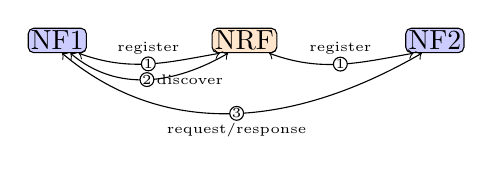
\begin{tikzpicture}[nf/.style={draw, rounded corners=2pt, fill=blue!20, inner sep=1pt},
lab/.style={circle, draw, fill=white,minimum width=5pt,inner sep=0}]
	\node[nf] at (0,0) (nf1) {NF1};
	\node[nf, fill=orange!20] at ([xshift=2cm]nf1.east) (nrf) {NRF};
	\node[nf] at ([xshift=2cm]nrf.east) (nf2) {NF2};
	\draw[<->] ([xshift=-3pt]nf1.south east) to[out=-20,in=190] coordinate (l1) ([xshift=3pt]nrf.south west);
	\draw[<->] ([xshift=-3pt]nrf.south east) to[out=-20,in=190] coordinate (l2) ([xshift=3pt]nf2.south west);
	\draw[<->] ([xshift=-6pt]nf1.south east) to[out=-40,in=210] coordinate (l3) ([xshift=6pt]nrf.south west);
	\draw[<->] ([xshift=-9pt]nf1.south east) to[out=-40,in=210] coordinate (l4) ([xshift=6pt]nf2.south west);
	\node[lab] at (l1) {\tiny 1};
	\node[lab] at (l2) {\tiny 1};
	\node[lab] at (l3) {\tiny 2};
	\node[lab] at (l4) {\tiny 3};
	\node[below] at (l4) {\tiny request/response};
	\node[right] at (l3) {\tiny discover};
	\node[above] at (l2) {\tiny register};
	\node[above] at (l1) {\tiny register};
\end{tikzpicture}

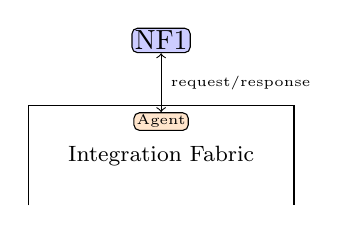
\begin{tikzpicture}[nf/.style={draw, rounded corners=2pt, fill=blue!20, inner sep=1pt},
lab/.style={circle, draw, fill=white,minimum width=5pt,inner sep=0}]
	\node[nf] at (0,0) (nf1) {NF1};
	
	\node[inner sep=0.5cm] at ([yshift=-1.3cm]nf1.south) (bsm) {\footnotesize Integration Fabric};
	\node[nf,fill=orange!20] at ([yshift=-0.2cm]bsm.north) (ag) {\tiny Agent};
	\draw (bsm.south west) -- (bsm.north west) -- (bsm.north east) -- (bsm.south east);
	\draw[<->] (nf1.south) -- node[right] {\tiny request/response} (ag.north);
\end{tikzpicture}


\section{Acknoledgements}
This work was supported by the ICT R\&D program of MSICT/IITP. [2021-0-02094, International collaborative research on 6G network architecture and core technologies]

\section{References}

\begin{comment}
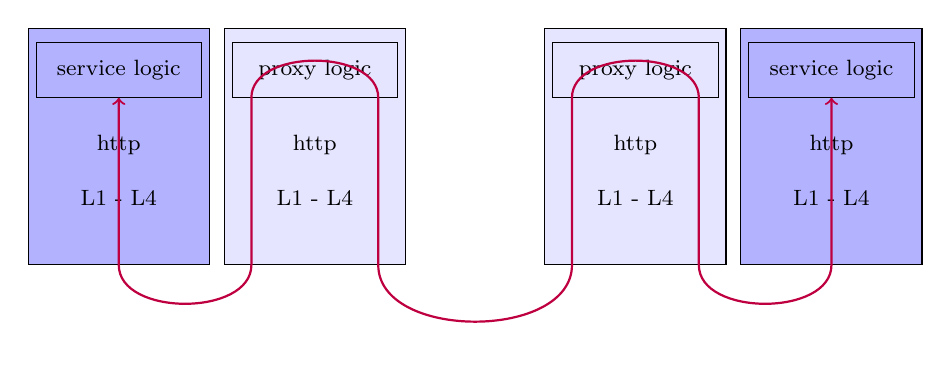
\begin{tikzpicture}[bound/.style={draw=black,rectangle, minimum width=2.3cm, minimum height=3cm,fill=blue!10},
log/.style={rectangle,draw=black, minimum width=2.1cm, minimum height=0.7cm, inner sep=2pt, align=center,font=\footnotesize}]
	\node[bound,fill=blue!30] at (0,0) (b1) {};
	\node[bound,right] at ([xshift=5pt]b1.east) (b2) {};
	\node[bound,right] at ([xshift=50pt]b2.east) (b3) {};
	\node[bound,fill=blue!30,right] at ([xshift=5pt]b3.east) (b4) {};
	
	\node[log,below] at ([yshift=-5pt]b1.north) (m1) {service logic};
	\node[log,below] at ([yshift=-5pt]b2.north) (m2) {proxy logic};
	\node[log,below] at ([yshift=-5pt]b3.north) (m3) {proxy logic};
	\node[log,below] at ([yshift=-5pt]b4.north) (m4) {service logic};
	\node[below] at ([yshift=-10pt]m1.south) {\footnotesize http};
	\node[below] at ([yshift=-30pt]m1.south) {\footnotesize L1 - L4};
	\node[below] at ([yshift=-10pt]m2.south) {\footnotesize http};
	\node[below] at ([yshift=-30pt]m2.south) {\footnotesize L1 - L4};
	\node[below] at ([yshift=-10pt]m3.south) {\footnotesize http};
	\node[below] at ([yshift=-30pt]m3.south) {\footnotesize L1 - L4};
	\node[below] at ([yshift=-10pt]m4.south) {\footnotesize http};
	\node[below] at ([yshift=-30pt]m4.south) {\footnotesize L1 - L4};
	\coordinate (p1) at ([xshift=10pt]b2.south west);
	\coordinate (p2) at ([xshift=-10pt]b2.south east);
	\coordinate (p3) at ([xshift=10pt]b3.south west);
	\coordinate (p4) at ([xshift=-10pt]b3.south east);
	
	\draw[<->,thick,purple] (m1) -- (b1.south) to[out=-90,in=-90] (p1) -- (p1 |-m2.south) to[out=90,in=90] (p2 |- m2.south) -- (p2) to[out=-90,in=-90] (p3) -- (p3 |- m3.south) to[out=90,in=90] (p4|-m3.south) -- (p4) to[out=-90,in=-90] (b4.south) -- (m4);
\end{tikzpicture}
\end{comment}

\end{document}